\section{Research Area Introduction}
\label{sec:Research area introduction}

In this section, the details of various approaches and the \ac{sota} in 3D \ac{hpe} are presented along with some works in the sibling tasks of hand pose estimation. This section aims to only give an overview of how the problem of 3D \ac{hpe} is tackled in the literature, approaches that are directly related to the method proposed in this thesis are presented later in section \ref{sec:Related Work}, Related Works. The different categories of the approaches mentioned below are not exclusive but are the main aspects of the described approaches.

\subsection{Cascading Approach}

Numerous works try to estimate 3D human poses from 2D RGB images or 2D joint confidence heatmaps \cite{CameraDistanceAware, poselifter, DistillNRSfM, occlusionVideo, ordinalranking}. Most of these methods follow a cascading approach, where an explicit intermediate representation of 2D heatmaps or 2D poses are predicted. This typically involves training a convolutional neural network to find humans in the image or just extract features that correspond to the joints. These features are forwarded to another neural network that learns to estimate the corresponding 3D pose, usually by predicting the depth offsets of the 2D joint or sometimes by predicting the shape and the view parameters of the 3D pose.

For example, \cite{CameraDistanceAware} proposes a general framework with 3 networks as depicted in Fig \ref{fig:CameraDistanceAware}. Human detection Network, RootNet, PoseNet. Where the human detection network predicts the region the human is in an image. The RootNet localizes the human's root in the global 3D world. And, the PoseNet predicts the 3D pose of a single person relative to the root. Where the root is a fixed reference point of the human body say, pelvis.

\begin{figure}[h]
    \centering
    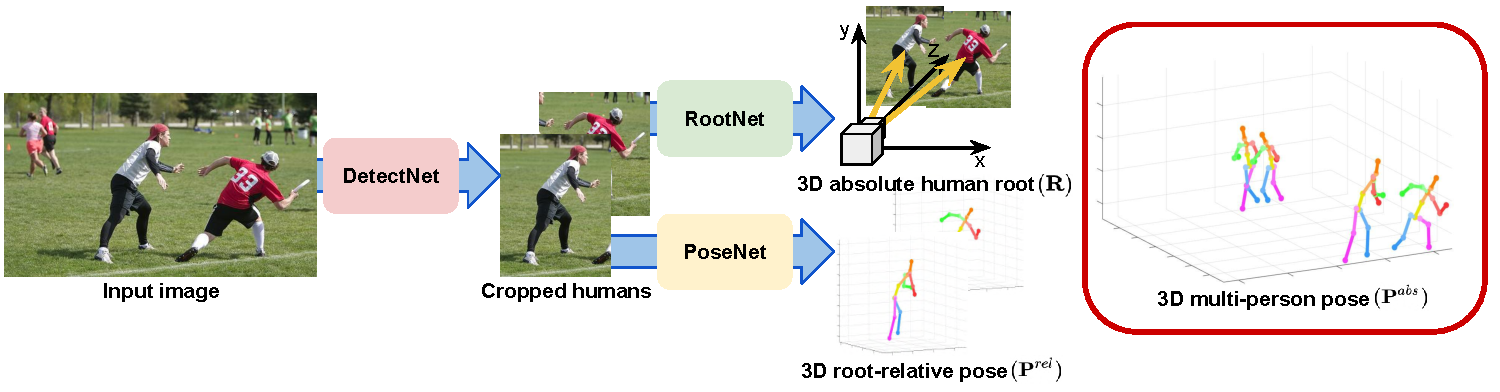
\includegraphics[width=\linewidth]{figures/background/cascading_arch.pdf}
    \caption{Pipeline of an absolute 3D human pose estimation network following a cascading approach \cite{CameraDistanceAware}, showing different neural networks such as DetectNet, RootNet and PoseNet that trained on specific subtasks to estimate absolute 3D human pose.}
    \label{fig:CameraDistanceAware}
\end{figure}

The advantage of such top-down frameworks is the possibility to divide the task of RGB to 3D into smaller, well-studied sub-tasks. This enables explicit supervision of know intermediate states that could be on interest for undestanding the representations learned by the network or to use the intermediate output for other auxilary tasks. Moreovere, in this case it makes scaling single-person pose estimation algorithms for multi-person pose estimation easy, as the majority of the data available mostly consists of a single person per frame. Most importantly certain modules can be replaced or improvised without affecting or having to re-train the entire pipeline.

\subsection{Pose Lifting}

In contrast to the estimating pose from an image, Pose Lifting works such as \cite{poselifter,  amazon1, repnet, c3dpo, unsupervisedAdversarial}, focus on estimating 3D poses from 2D poses alone while assuming 2D poses from the \ac{sota} methods in 2D \ac{hpe}. This category follows the idealogy of cascading based approaches but restricts the study and discussion purely to lifting 2D to 3D pose. These methods include simple linear models as first described in \cite{MartinezHRL17} with a series of fully connected linear, batch normalization, dropout layers with residual connections  as illustrated in Fig \ref{fig:lifting_arch} to regress 3D pose effectively. These simple networks have enough capability to capture the features of the data as the input and output data are much smaller in dimensions as compared to RGB images.

\begin{figure}[h]
    \centering
    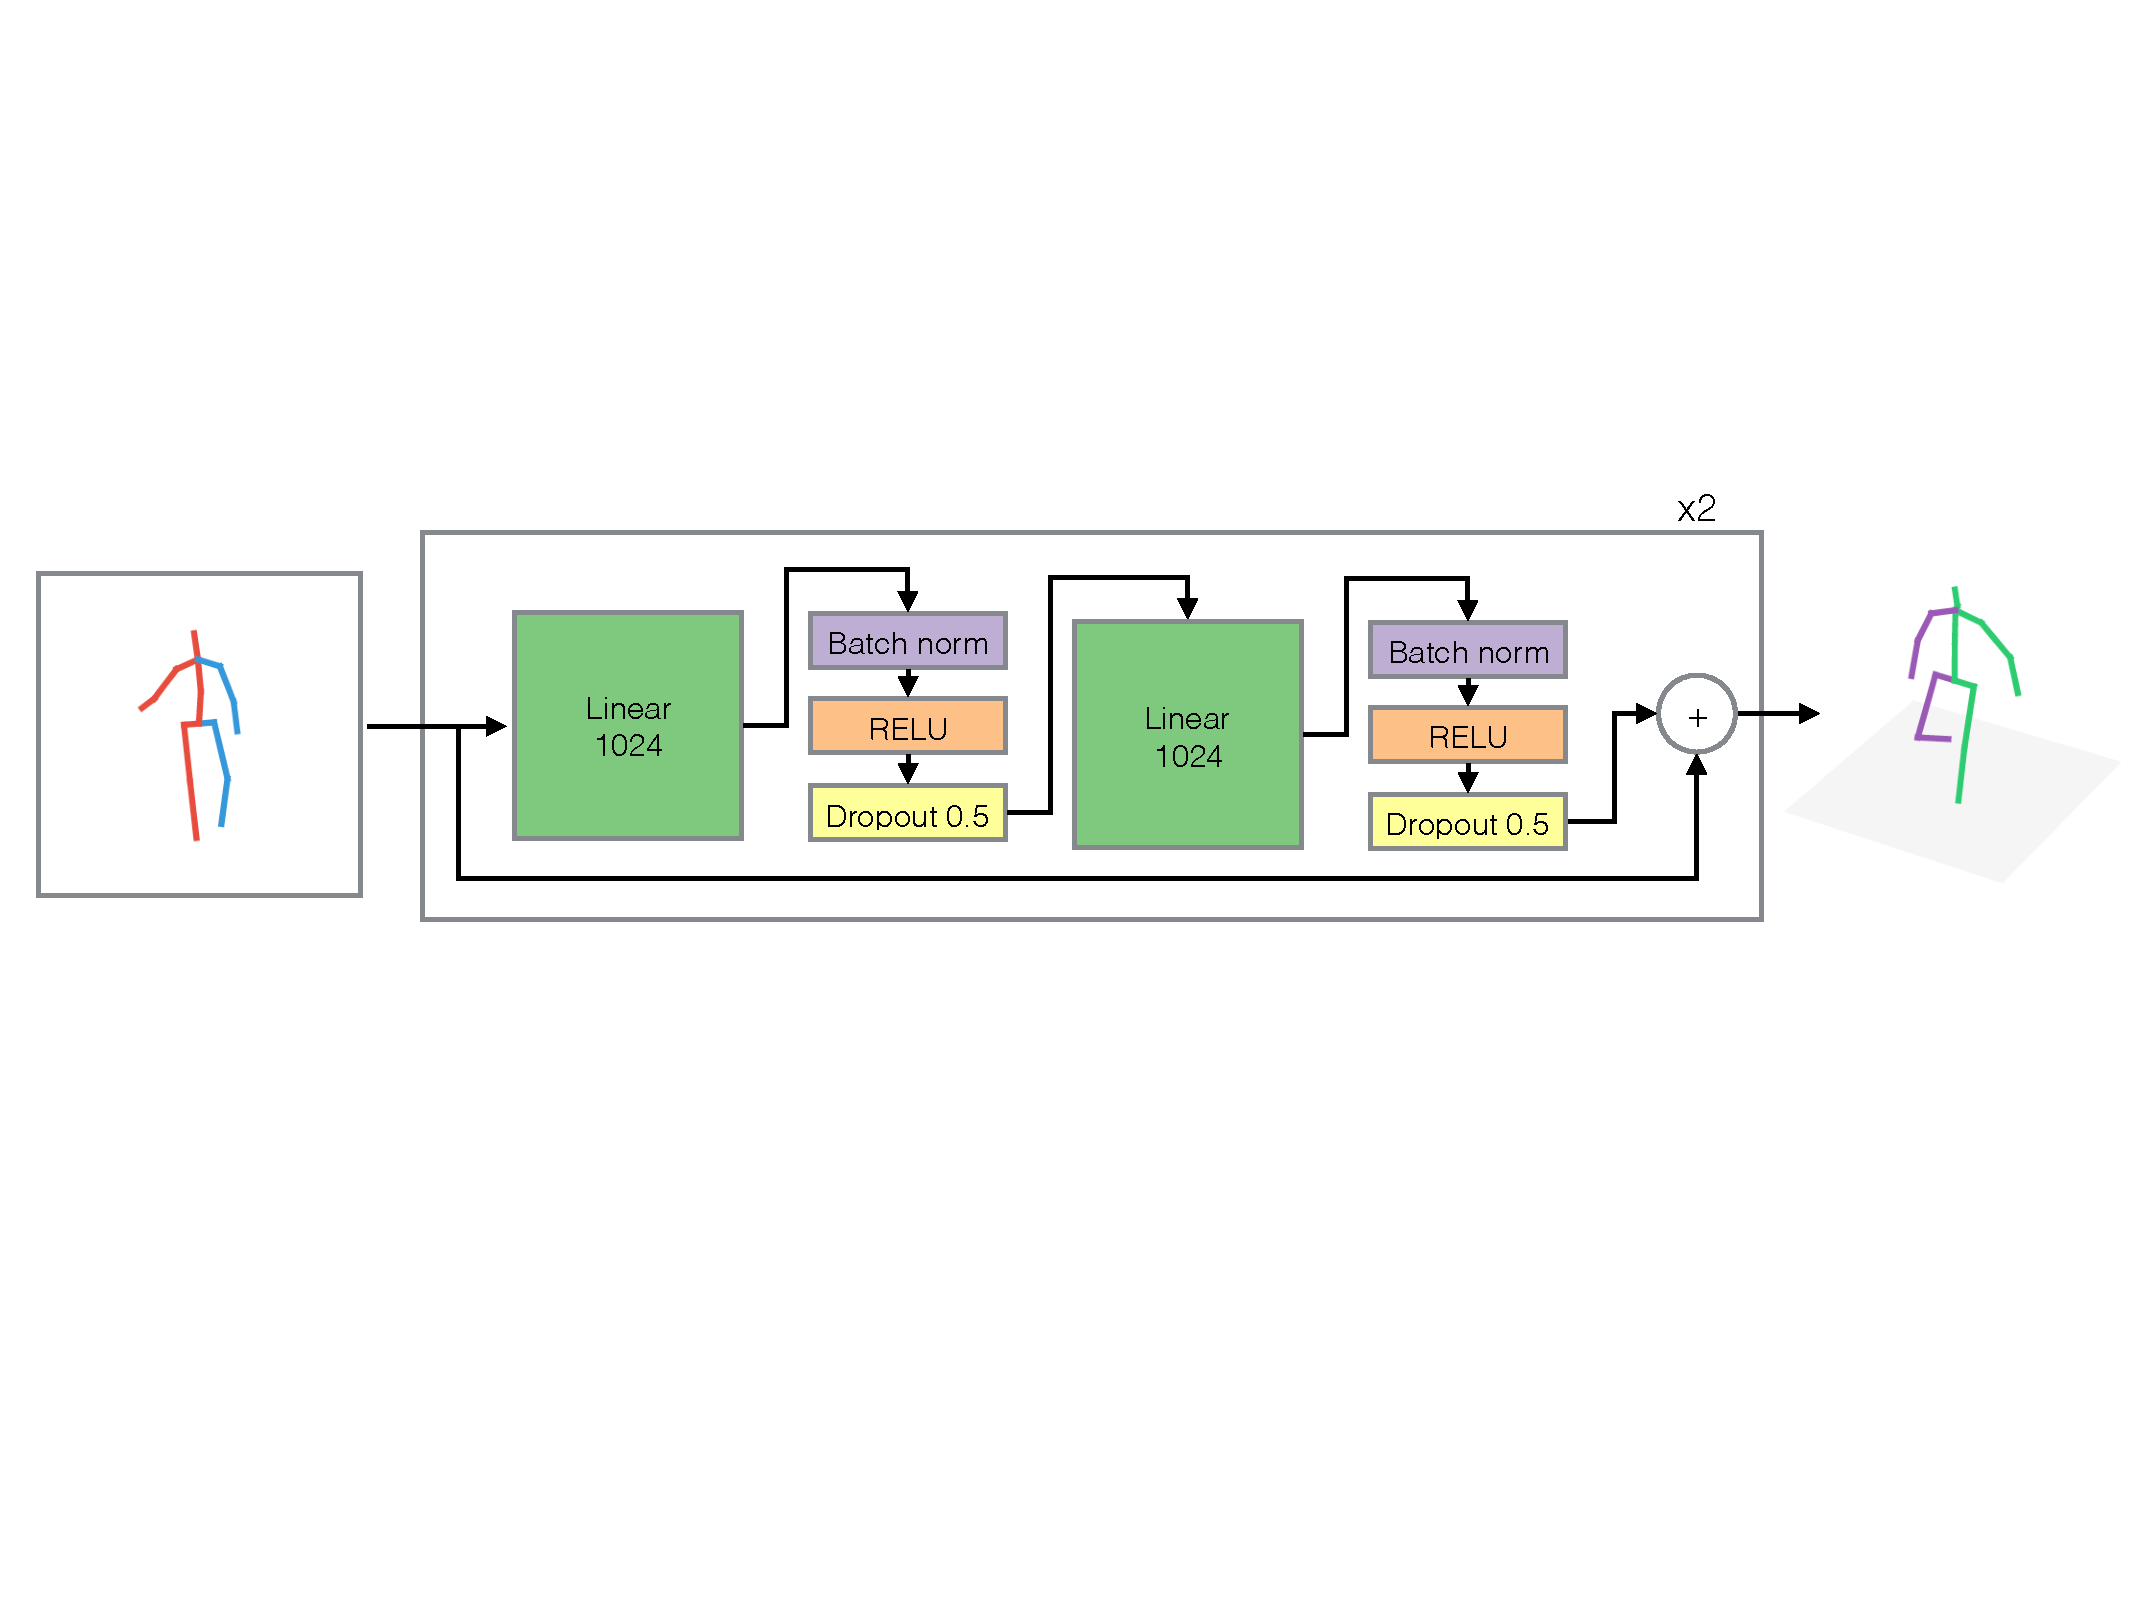
\includegraphics[width=\linewidth]{figures/background/lifting_arch.pdf}
    \caption{Architecture of the first deep learning based lifting appraoch proposed by Martinez \textit{et al.} \cite{MartinezHRL17}}
    \label{fig:lifting_arch}
\end{figure}

\ac{nrsfm} is another promising lifting method that also leverages images along with 2D annotations. \ac{nrsfm} deals with the problem of reconstructing 3D shape (pose/point cloud) and cameras of each projection from a sequence of images with corresponding 2D projections (2D keypoints). This approach has been widely used in facial keypoint detection and \cite{deepNRSFM} introduces deep learning variant for the same. Instead of predicting the 3D coordinates of each keypoint/joint of the 3D pose, \cite{DistillNRSfM, c3dpo, deepNRSFM, nrsfm++} predicts the 3D shape and camera pose from 2D pose using this method. The advantage of such approach is to obtain disentagled representation of view and 3D pose that is invariant of the view or camera position.

The Lifting approaches facilitate to leverage the already well established 2D \ac{hpe} models that are trained on enormous and diverse labeled data. Thus demanding lesser training data for 3D pose estimation than it would need when learning from images. Since these networks do not have large convolution layers they are computationally inexpensive for both training and inference. Moreover, the 2D and 3D pose data usually can be entirely loaded onto the GPU further accelerating the training procedure. Thus addressing one of the major problems that effects the scalability of 3D \ac{hpe} models as well as enabling the development of better modular systems by combining the best of Lifting networks with the best of 2D \ac{hpe}.

\subsection{Multiple Hypothesis Estimation}
\label{subsec:multiple_hypothesis_estimation}

As stated in \ref{sec:background}, 2D-to-3D pose lifting is an ill-posed-inversed problem due to inherent depth ambiguity as there are multiple plausible 3D poses that gives the same 2D projection, this shall be further eloborated later in chapter \ref{chap:data}, Data. To address this problem, Jahangiri \textit{et al.} \cite{jahangiri} propose a solution a 3D \ac{gmm} to learn uniformly sampled 3D poses and canditionally sample to retrieve 3D poses that have the reprojection error within the given limits. Thus estimating multiple 3D poses conditioning on a single input 2D pose, similar to a dictionary based learning approach. 

More deep learning based approaches such as \cite{weaklymultiple,multiplehypo,ordinalranking} were later inroduced. Out of them, Chen Li \textit{et al.} \cite{multiplehypo} proposes a variational inference model replacing the \ac{gmm} with a \ac{mdn} which was first introduced by Ye \textit{et al.} \cite{mixturedensitymodel} to handle occlusions in hand pose estimation. Thus addressing two of the major problems of 3D \ac{hpe} i.e missing joints from occlusions and variational inference. 

Another interesting approach from Sharma \textit{et al.} \cite{ordinalranking}, presents a conditional \acl{vae} which takes a random sample from a normal distinguish as an input and 2D pose as a condition and outputs different 3D pose for different random samples given the same 2D pose. This approach also handles missing joints and provides variational inference. A evaluation technique is also proposed to rank each of the multiple hypotheses by scoring the poses based on joint-ordinal depth relations learnt from the images or by oracle score that access 3D ground truth to comptute the closest match as illustrated in Fig \ref{fig:ordinal_arch}.

\begin{figure}[h]
    \centering
    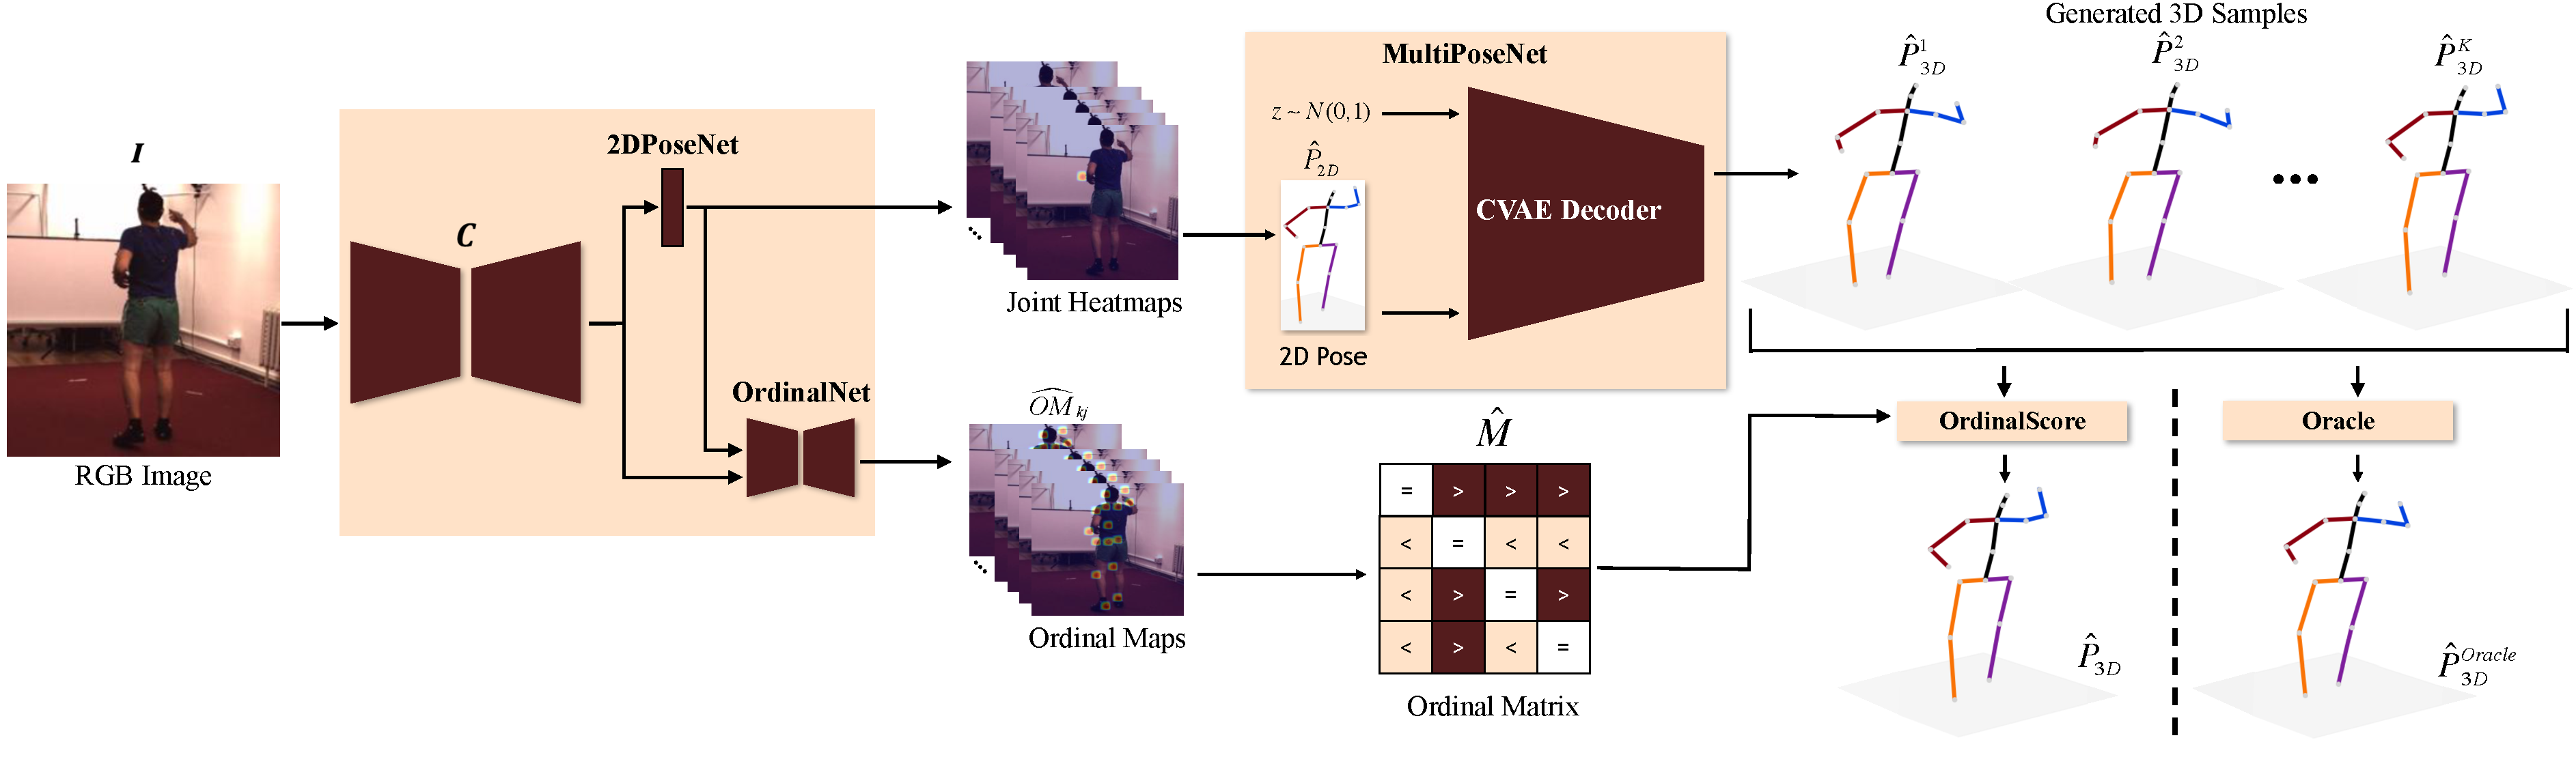
\includegraphics[width=\linewidth]{figures/background/ordinal_arch.pdf}
    \caption{Illustration of modular framework from \cite{ordinalranking} that uses a Conditional \ac{vae} to estiamte multiple hypothesis for a given 2D pose as condition. The ordinal scoring learnt from joint-depth ordinal relations and the score obtained from the oracle that learns scores higher to poses closest to the ground truth pose are used rank to each of the predicted 3D pose.}
    \label{fig:ordinal_arch}
\end{figure}

Recent work from Chen Li \textit{et al.} \cite{weaklymultiple} which is an improvised version of their earlier work \cite{multiplehypo} proposes a weakly supervised approach that is much more similar to that of this thesis. The details are discussed later in related works section \ref{sec:Related Work}. However, all of the mentioned appraoches still require 3D poses in one way or other for training and hence do not address the most important bottleneck of obtaining 3D ground truth. 

\subsection{Non-Supervised Learning}
\label{subsec:non_supervised_learning}
The standard way to train 3D/2D \ac{hpe} is by minimizing the distance between the predicted 3D/2D pose and its corresponding 3D ground truth. The area of 2D \ac{hpe} is well established and matured with reliable systems deployed in the real world. This was made possible with the high volume of images from diverse settings and the reasonable ease of manual labeling of 2D poses. On the other hand, labeling 3D pose manually is not practical. Though single-person datasets such as Human3.6M \cite{H3.6}, Human Eva \cite{HumanEva} and, multi-person datasets such as CMU Panoptic \cite{cmuPanoptic} provide 3D pose ground truth, they are obtained using \ac{mocap} systems Fig[\ref{fig:h36_mocap}] which are only limited to indoors or cannot be directly adapted to outdoor environments where the majority of the use cases exist. It is also worth mentioning JTA (Joint Track Auto) dataset \cite{JTA} that is made using the GTA(Grand Theft Auto) game engine which is technically scalable with its own limitations. The datasets from simulations come with the difficulty of domain adaptation to be transferable to the real world.

\begin{figure}[h]
    \centering
    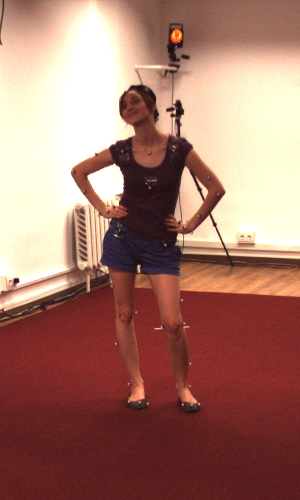
\includegraphics[width=30mm]{figures/h36/h36_mocap.png}
    \caption{Image from Human3.6 Dataset \cite{H3.6} of subject wearing \ac{mocap} markers}
    \label{fig:h36_mocap}
\end{figure}

To overcome this bottleneck, \cite{unsupervisedAdversarial} proposes unsupervised training of a generative adversarial network by projecting the predicted 3D pose back to 2D and minimizing its distance with the input 2D pose. And further training a discriminator to distinguish the real 2D pose from the projected poses as illustrated in Fig \ref{fig:adverserial_arch}. Thus removing the need for any explicit 3D annotations besides 2D pose that are either manually labeled or obtained using 2D \ac{hpe} models. RepNet \cite{repnet} trains an adversarial network without 2D-3D correspondences in a weakly supervised manner. Moreover, it also does not require camera parameters to project the 3D pose but learns to predict them. Thus enabling better generalization to more diverse data with unknown cameras and poses.

\begin{figure}[h]
    \centering
    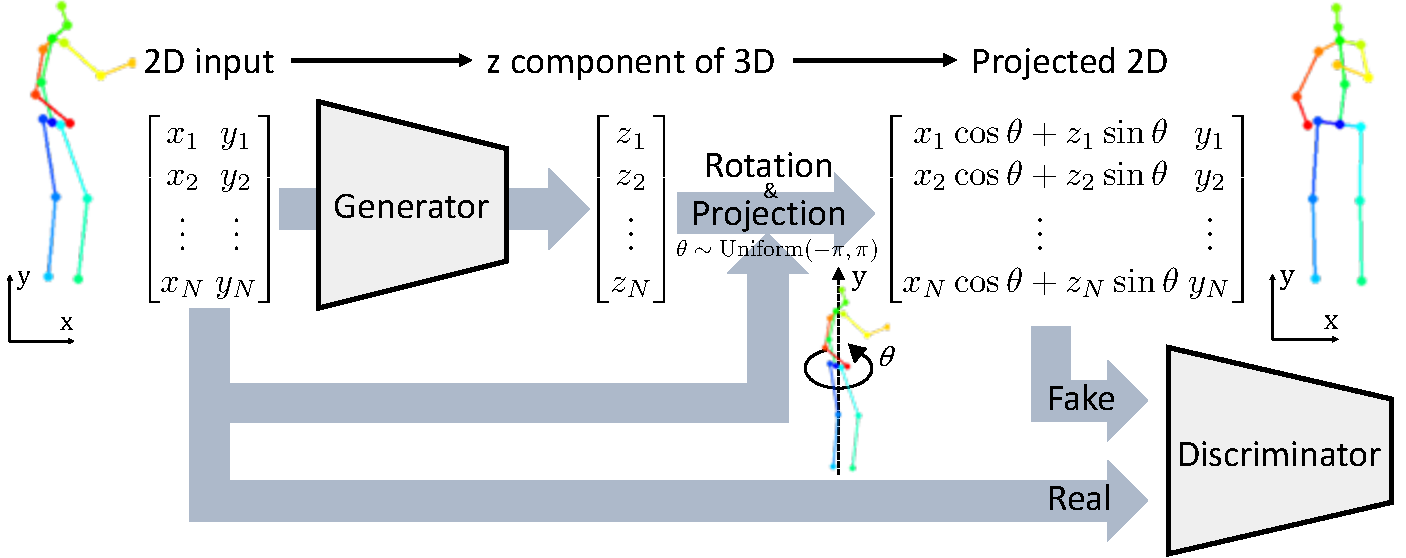
\includegraphics[width=\linewidth]{figures/background/adverserial_arch.pdf}
    \caption{Architecture of a simple unsupervised adversarial learning architecture proposed by \cite{unsupervisedAdversarial}. The network takes 2D coordinates ($x$, $y$) of each joint in the pose and predicts the corresponding $z$-component. The 3D pose achieved by combining the input $x$, $y$ with the predicted $z$, is the randomly rotated along the $y$-axis to retrieve a novel view of the 3D pose. This pose is the projected to $xy$-plane, which would be much differnet from the input 2D pose. This projected 2D pose should be similar to the real 2D poses in the dataset if the predicted 3D represents true human pose. Their similarity to real 2D poses is reinforced by a discriminator. The whole trianing produce is carried out without the need for 3D pose in any shape or form.}
    \label{fig:adverserial_arch}
\end{figure}

To test the maximum capability of Pose Lifting networks, \cite{amazon1} proposes a combination of unsupervised and adversarial learning that mainly leverages the property of \textit{plane-invariance}. It is the property that 2D projections of a 3D pose from different camera viewpoints, when lifted should produce identical and the original 3D pose. In this method, the predicted 3D pose is rotated in random angles and is reprojected to 2D in a different \ac{pov}. A discriminator is then used to evaluate if this new 2D pose is in the possible pose distribution which is learned from 2D pose datasets alone. These steps are redone in reverse order to obtain the original 2D input. This cycle provides three intermediate representations of the single 2D input that the models learn from. Additionally, this approach exploits the temporal consistency in the datasets as well as integrates a domain adaptation network to learn from different datasets and distributions to achieve comparable results to that of the methods that require more supervision. However, due to the inherent ambiguity in lifting 2D pose to 3D and as the images are not captured with orthogonal cameras, reprojection of 3D pose is not neccessarily consistent with the ground truth as the camera intrincsic and extrinsic parameters are not taken into account. Hence it is challenging to match the performance of models trained on 3D ground truth.

\subsection{Multimodal Representation Learning}
\label{subsec:multimodal_representation_learning}

Another interesting approach is training \ac{vae}s using multiple modalities like images, poses, depth maps \cite{CrossingNets, crossmodal, MMVAE,HandDisentangled}. \ac{mvae}s learn representation from different modalities in the same latent space. True multimodal learning needs to fulfill 4 criteria as follows: i) \textit{Latent Factorization} - Implicit factorization of latent space into private, shared subspaces based on modality as illustrated in the figure[\ref{fig:criteria}]. ii) \textit{Coherent Joint Generation} - Coherence in generations of different modalities from the same latent value with respect to the shared aspects of the latent. iii) \textit{Coherent Cross Generation} - Generation of one modality conditioned on data from different modality while preserving the similarity between them. iv) \textit{Synergy} - Enhancement in generation quality of one modality as a result of learning representations of different modalities.

\begin{figure}[h]
    \centering
    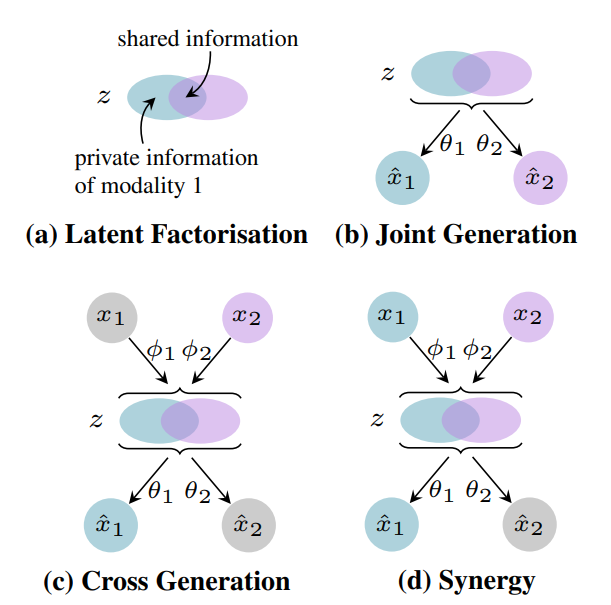
\includegraphics[scale=0.5]{figures/background/criteria.png}
    \caption{Criteria for Multimodal Generation \cite{MMVAE}}
    \label{fig:criteria}
\end{figure}

\ac{mmvae} proposed by \cite{MMVAE} fulfills all 4 of the above-mentioned criteria learning representations of image and text data, while other approaches focus on leveraging specific advantages of multimodal learning. Consider the cross-modal learning for 3D Hand Pose Estimation proposed by \cite{crossmodal}. It involves training an encoder-decoder pair to learn image representation, and another such pair to learn 3D hand pose representations in the same latent space. This training procedure focuses on cross-generation and synergy. That is, using the shared latent space of the image and pose representations, the RGB image encoder combined with the pose decoder can generate 3D poses and vice versa while preserving the commonality between the conditioned and the generated data. With this approach, it is possible to train a \ac{vae} for 3D \ac{hpe} from RGB images without explicit intermediate stages like the earlier mentioned cascading approaches. Making it more efficient and fast for both training and inference without compromising the modularity offered by cascading approaches.

\section{Related Work}
\label{sec:Related Work}

In this section, works that are directly related to the thesis are discussed in more detail. Some are the best examples of their kind and have already been discussed thoroughly. The basic idea of the thesis is to learn 3D \ac{hpe} just from 2D pose data without using 3D ground truth in any shape or form. Thus developing a method that can exploit the huge amounts of 2D pose data that can be generated using state of the art 2D pose networks on diverse images from the real world. The following approaches use weakly supervised or unsupervised approaches to accomplish the same. These serve as the inspiration for many of the choices taken in this thesis and also help understand the possibilities of reducing the need for explicit 3D supervision.

To the best of knowledge acquired during the period of the thesis, \cite{can3dpose, amazon1, unsupervisedAdversarial, c3dpo} are the main approaches that do not use 3D supervision in any way. While \cite{repnet, weaklymultiple} are among the main approaches that use 3D supervision to train the discriminator alone. The approaches that are not mentioned are either the approaches the above mentioned are built up or have been missed during the literature study or most likely published after finishing this thesis report.

\cite{unsupervisedAdversarial, can3dpose, amazon1} can be viewed as a series of approaches that are built on one another in the same order. They take 2D poses as the input and learn to predict the depth offset for each joint to reconstruct 3D. Out of the three Ching \textit{et al.} \cite{amazon1}, using the plane invariance, geometric self-supervision, and adversarial learning as discussed earlier \ref{subsec:non_supervised_learning}, achieves the \ac{sota} results compared to fully supervised methods and also present ways to use domain adaptation network, temporal consistency to further integrate more datasets and improve the performance. Thus directly address the hurdles of scaling the 3D \ac{hpe} network to the real world. However, they also acknowledge the fact that most of the predictions made by \ac{sota} 2D \ac{hpe} model on real-world images have missing joints. Since the proposed approaches only predict the depth of every joint, the error from the 2D input pose is directly propagated to the 3D prediction. More importantly, it is not possible to use most of the data that is generated from 2D pose models. Hence it is very crucial to handle the problem of \textit{\textbf{missing joints}} to truly unlock the potential of unsupervised learning.

Wandt \textit{et al.} \cite{repnet} also mentioned in \ref{sec:Research area introduction} proposes an architecture that learns to predict the whole 3D pose, while also learning the camera parameters that are used to project the predict 3D to 2D. The idea behind the camera parameter network is to learn the view angle given pose to generalize to unknown cameras. The pose network learns to converge the predicted 2D reprojections, while using a \ac{gan} trained on \textit{\textbf{3D ground truth labels}} to supervise the predicted 3D pose. Though there is no direct error propagation from 2D input to 3D, it is important to note the problem of missing joints is not yet addressed. However, there another fundamental problem of \textit{\textbf{depth ambiguity}} persists. 

\begin{figure}[h]
    \centering
    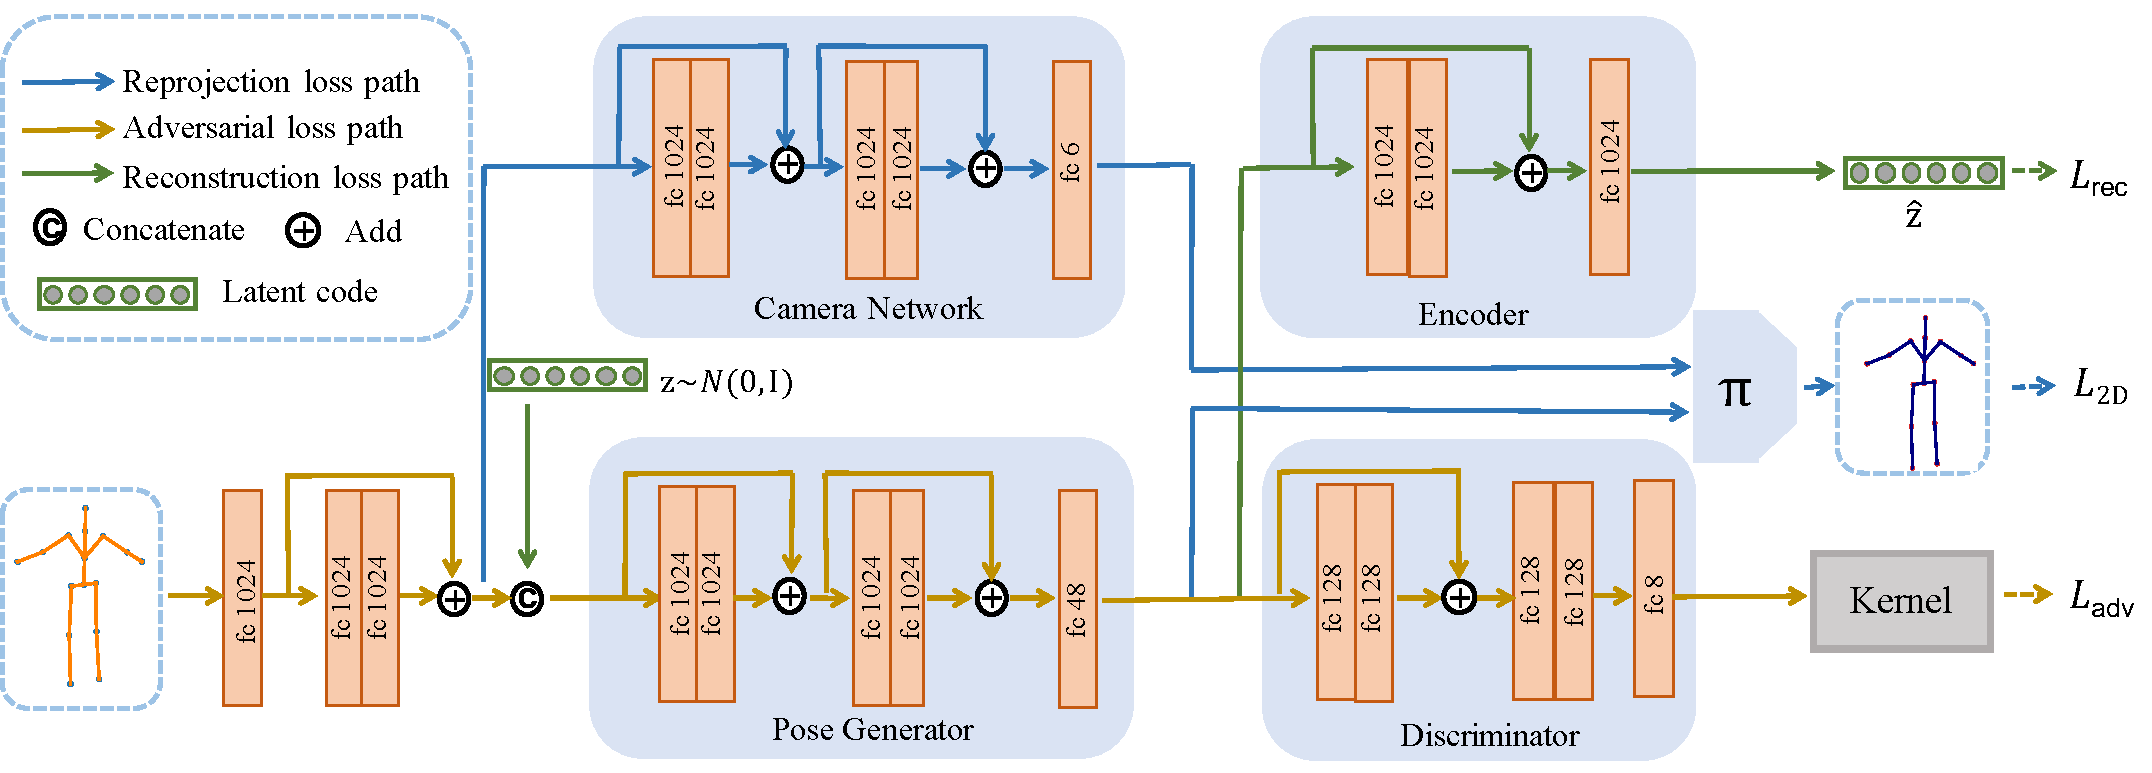
\includegraphics[width=\linewidth]{figures/background/multi_arch.pdf}
    \caption{Illustraion of the weakly supervised multiple hypothesis generation architecture proposed by \cite{weaklymultiple}}
    \label{fig:multi_arch}
\end{figure}


Chen Li \textit{et al.} \cite{weaklymultiple}, building upon their previous work \cite{multiplehypo} that is explained earlier in \ref{subsec:multiple_hypothesis_estimation}, proposes a weakly supervised variational inference model as the proposed method in this thesis was developed. The new approach \cite{weaklymultiple} was inspired by the architecture of Wandt \textit{et al.} \cite{repnet} that does not require direct 3D supervision. This model first encodes the input 2D pose to a latent representation. This representation is then concatenated with a \textit{latent code} to produce a 3D pose as well as used by the camera network to predict the camera pose. Instead of directly supervising the predicted 3D pose with the ground truth, it is projected back to 2D using the predicted camera view which is self supervised as it should be the same as the input 2D pose. 

This self supervision trains the network to only output 3D poses that are close to input 2D in a particular view but uncontrained from other view. To ensure, the predicted 3D is feasible and close to ground truth a \ac{wgan} is used as illustrated in Fig \ref{fig:multi_arch}. The predicted 3D pose is passed to a critic network that scores the poses on how realistic they are. This encourages the pose network to generate poses that are realistic, in other words indistingushable from the 3D ground truth poses. This results in a realistic 3D pose that is close to 2D input pose which is most likely close to its corresponding 3D ground truth. In addition to this an encoder is trained to reconstruct the latent code to ensure diversity and prevent mode collapse of the \ac{wgan}. 

This variational inference of 3D pose addresses both the problems of depth ambiguity and missing joints. However, this weakly supervised still requires 3D ground truth poses to train the discriminator and does not address the problem completely. The method proposed in this thesis is similar to this approach but does not require 3D in any shape or form, and uses much smaller architecture without the camera and latent vector encoder networks while addressing all the major problems. 

Canonical 3D Pose Networks for Non-Rigid Structure From Motion (C3DPO) \cite{c3dpo}, which is also discussed in \ref{subsec:non_supervised_learning} handles missing joint and is fully unsupervised but does not have the capability of predicting multiple hypotheses for a given 2D pose. This approach that uses \ac{nrsfm} in an unsupervised way, does not yield good results compared to other approaches. In this thesis, we present a method that has the meritcs of the above approaches and address all the aforementioned problems.